\documentclass[12pt,letterpaper, margin = 3cm]{article}
\footskip = 50pt
\topmargin = -3cm
\usepackage[spanish]{babel}
%\usepackage[ansinew]{inputenc}
\usepackage[utf8]{inputenc}
% \usepackage[latin1]{inputenc}
\usepackage[letterpaper,includeheadfoot, top=0.5cm, bottom=5.0cm, right=2.0cm, left=2.0cm]{geometry}
\renewcommand{\familydefault}{\sfdefault}

\usepackage{graphicx}
\usepackage{color}
\usepackage{hyperref}
\usepackage{amssymb}
\usepackage{url}
%\usepackage{pdfpages}
\usepackage{fancyhdr}
\usepackage{hyperref}
\usepackage{subfig}

\usepackage{listings} %Codigo
\definecolor{dkgreen}{rgb}{0,0.6,0}
\definecolor{gray}{rgb}{0.5,0.5,0.5}
\definecolor{mauve}{rgb}{0.58,0,0.82}

\lstset{
  language=Java,
  aboveskip=3mm,
  belowskip=3mm,
  showstringspaces=false,
  columns=flexible,
  basicstyle={\small\ttfamily},
  numbers=none,
  numberstyle=\tiny\color{gray},
  keywordstyle=\color{mauve},
  commentstyle=\color{blue},
  stringstyle=\color{dkgreen},
  breaklines=true,
  breakatwhitespace=true
  tabsize=3
}

\begin{document}
%\begin{sf}
% --------------- ---------PORTADA --------------------------------------------
\newpage
\pagestyle{fancy}
\fancyhf{}
%-------------------- CABECERA ---------------------
\fancyhead[L]{ 
\includegraphics[scale=0.09]{img/logodcc.png} }
%------------------ TÍTULO -----------------------
\vspace*{5cm}
\begin{center}
\huge  {Tarea 3}\\
\Huge {Euclidean Travelling Salesman Problem}\\
\vspace{6cm}
\end{center}
%----------------- NOMBRES ------------------------
\vfill
\begin{flushright}
\begin{tabular}{ll}
Autores: & Claudio Berroeta\\
& Sebastián Ferrada \\
Profesor: & Pablo Barceló\\
Auxiliar: & Miguel Romero\\
Ayudantes: & Javiera Born\\
& Giselle Font\\
& \today\\
\end{tabular}
\end{flushright}

% ·············· ENCABEZADO - PIE DE PAGINA ············
\newpage
\pagestyle{fancy}
\fancyhf{}

%Encabezado
%\fancyhead[L]{\rightmark}
\fancyhead[L]{\small \rm \textit{Sección \rightmark}} %Izquierda
\fancyhead[R]{\small \rm \textbf{\thepage}} %Derecha


\fancyfoot[C]{\small \rm \textit{Euclidean Travelling Salesman Problem\\}} %Izquierda
%\fancyfoot[R]{\small \rm \textit{Pie de página - Derecha}} %Derecha
%\fancyfoot[C]{\thepage} %Centro

\renewcommand{\sectionmark}[1]{\markright{\thesection.\ #1}}
\renewcommand{\headrulewidth}{0.5pt}
\renewcommand{\footrulewidth}{0.5pt}
\newcommand{\fancyfootnotetext}[2]{%
  \fancypagestyle{dingens}{%
    \fancyfoot[LO,RE]{\parbox{12cm}{\footnotemark[#1]\footnotesize #2}}%
  }%
  \thispagestyle{dingens}%
}

% =============== INDICE ===============

\tableofcontents
%\listoffigures

% =============== SECCION ===============
\newpage
\section{Introducción}

% ----- Texto Introducción------
En el presente informe se pretende mostrar un análisis sobre la performance de distintas aproximaciones para resolver el problema del vendedor viajero. Este problema requiere un recorrido hamilnoniano tal que el vendedor visite las ciudades de un país solo una vez, recorriendo la menor distancia posible. Es bien conocido que la resolución de este problema de forma óptima es $NP-Hard$, i.e., toma tiempo exponencial.\\
A continuación, se revisarán 3 formas de aproximarse a este problema. La primera de ellas utiliza Minimum Spanning Trees sobre un grafo completo, en el cual cada ciudad es un nodo, y el peso de las aristas corresponde a la distancia de las ciudades. Luego, se recorre el árbol construído en preorden y se tiene un circuito de largo a lo más 2 veces el óptimo.\\
Otra aproximación consiste en ir desde cada ciudad, a la ciudad más cercana. Esta también es una 2-aproximación al problema.\\
Finalmente, se estudiará la performance de una heurística, es decir, un algoritmo que suele funcionar bien, pero que no entrega garantías sobre sus resultados, por lo que pueden llegar a ser bastante malos en ciertas ocaciones. Esta heurística calcula la envoltura convexa sobre las ciudades y luego se buscan puntos que minimicen ciertas distancias y se van agregando al circuíto.\\
Además de revisar cuántas veces más distancia se recorre con los algoritmos respecto al óptimo, se medirán los tiempos que toma la ejecución de estos.
% ----------------------------------

\subsection{Hipótesis}
\begin{enumerate}
\item Se busca comprobar que las aproximaciones por MST y por punto más cercano sean una 2-aproximación al problema, es decir, que \[ \frac{ALG(x)}{OPT(x)}\leq 2 \]
\item Se espera que la heurística de envoltura convexa funcione bastante bien para estos casos, siendo entre 3 y 4 veces el óptimo. Aunque también puede suceder que las soluciones empeoren al aumentar la cantidad de puntos.
\item Las aproximaciones formales deben tomar bastante tiempo, del orden de $n^2$, MST por las operaciones de grafos (crear grafo completo y calcular todas las distancias) y punto más cercano debido a que compara los puntos en el circuito con las que no, $n$ veces.
\item La heurística de envoltura convexa debe tomar tiempo $O(n\log(n))$, pues el algoritmo para encontrar la envoltura toma tiempo de ese orden y luego entrar los arcos y puntos que minimizan las relaciones toma $O(n)$. 
\end{enumerate}

\subsection{Ambiente Operacional}
Los experimentos fueron ejecutados en un Notebook con Sistema Operativo Windows 8 de 64 bits, 8 Gb de
memoria RAM y procesador intel Core i7 de 3.630 GHz. Para la implementación se utilizó el Java Development Kit v1.7.

\newpage
\section{Diseño de las Aproximaciones y Experimentos}
Cada aproximación será implementada por una clase que extienda de la interfaz \verb+EuclideanTSPResolver+ cuyo método recibirá la lista de puntos debidamente leídos desde los archivos indicados\footnote{\url{http://www.math.uwaterloo.ca/tsp/world/countries.html}} y deben retornar un circuito hamiltoniano que incluya todos los puntos recibidos. Estos circuitos fueron implementados como listas enlazadas circulares.

\subsection{Aproximación por Punto más Cercano}
El algoritmo comienza con un conjunto de puntos P y el algoritmo se ejecuta de ls siguiente forma:
\begin{enumerate}
\item Se inicia el circuito C con un sólo punto de P, escogido arbitrariamente.
\item En cada paso se identifica el punto p que no pertenece a C, cuya distancia a cualquier punto de C es mínima. Formalmente:
 \[ p\not\in{C},\;\; \min_{q'\in{C}} dist(p,q') \] Extendemos el circuito C, de tal forma de que el punto encontrado esté exactamente después del punto con que minimiza la distancia.
\item Si no quedan puntos en el circuito C, se retorna C.
\end{enumerate}

Para correr los experimentos se utilizó una Array para representar las distancias entre cada punto que esté en P. Aquí es fundamental tener cuidado con el tamaño del Array, ya que este puede superar fácilmente el límite del heap size. Por ello se intento reducir la cantidad de memoria basándonos en que la matriz de adyacencia es simétrica, entonces se llevó a cabo el cálculo de todas las distancias ordenadas estratégicamente.\\ \\
Se utilizaron 2 listas para manejar los puntos: $Puntos$ $ visitados$ y $Puntos$ $por$ $visitar$.
Luego se escoge un punto arbitrario: se añade a  $Puntos$ $ visitados$, se elimina de $Puntos por visita$r y se inicia el circuito con ese punto (Notar que  $Puntos$ $ visitados$ y el circuito son equivalentes). \\ \\
En cada paso se añade el punto que minimiza la distancia a los puntos del circuito a la primera lista y se elimina el mismo de la segunda. Luego se añade ese punto al circuito.\\ \\
El algoritmo termina cuando la lista de$Puntos$ $por$ $visitar$r esté vacía, por ende el circuito va a estar completo.

\subsection{Aproximación por Envoltura Convexa}

Esta heurística, comienza con un circuito representado por la envoltura convexa del conjunto de ciudades. Esta envoltura se obtiene utilizando un recurso provisto en internet y que puede ser encontrado en \url{https://code.google.com/p/convex-hull/source/browse/Convex+Hull}. Particularmente, se utilizó la clase \verb+FastConvexHull.java+.\\
Una vez obtenido ese circuíto, se itera por el resto de las ciudades interiores a la enovltura, y por cada ciudad $p$, se busca el arco $(p1,p2)$ (obtenemos el puntero al vértice que contiene a $p1$) en el circuíto que minimiza la expresión \[ dist(p,p1)+dist(p,p2)-dist(p1,p2) \] luego, entre todos los puntos que aun no están en el circuíto, se busca aquel $p^*$ que minimiza \[ \frac{dist(p^*,p1)+dist(p^*,p2)}{dist(p1,p2)} \] entonces se agrega este $p^*$ al circuíto, entre $p1$ y $p2$, lo que es fácil, pues ya tenemos el puntero hacia $p1$ y agregar un elemento entre dos vértices es $O(1)$ pues nuestros circuitos hamiltonianos son listas enlazadas.\\
El código de búsqueda de los arcos y puntos que minimizan las relaciones puede encontrarse en los anexos.


\subsection{Diseño de los Experimentos}
Los experimentos consisten en ejecutar las aproximaciones sobre los datos de los diferentes países y para cada uno de ellos, calcular el ratio $\frac{ALG(x)}{OPT(x)}$ donde $F(x)$ es la distancia recorrida por el algoritmo $F$ sobre las ciudades de $x$. Por lo tanto, este ratio nos dice cuántas veces el óptimo es capaz de conseguir nuestra aproximación.\\
Además se medirán los tiempos de ejecución de cada aproximación, sobre cada set de datos, así podremos ver el \textit{trade off} que existe entre obtener una mejor solución y el tiempo requerido para obtenerla.

\newpage
\section{Resultados}
Se revisarán los resultados para cada aproximación, mirando cómo varían el tiempo y la distancia recorrida  en función de la cantidad de puntos que posee cada país, de marera que se puedan comprobar o desechar las hipótesis planteadas en el comienzo.

\subsection{Resultados Envoltura Convexa}
Como se dijo al comienzo, para cada algoritmo, mediremos dos variables, tiempo de ejecución y distancia del circuito entregada por el algoritmo.

 \begin{figure}[ht!]
 \centering
 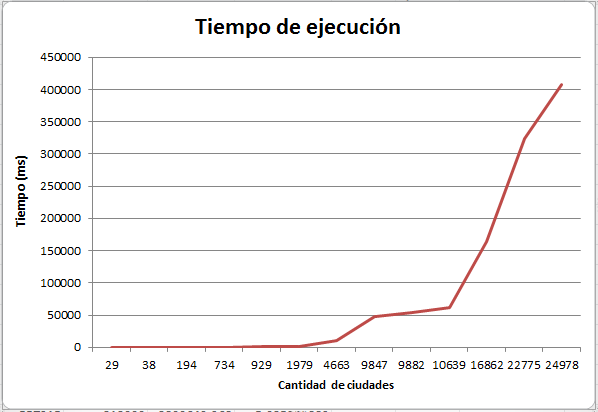
\includegraphics[scale=0.8]{img/timeconvexH.png}
 \caption{Tiempo de ejecución vs. Cantidad de ciudades}
 \end{figure}
%··········································
 \begin{figure}[ht!]
 \centering
 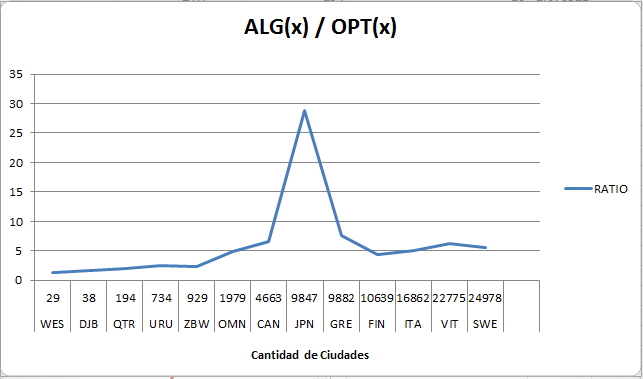
\includegraphics[scale=0.8]{img/ratioconvexH.png}
 \caption{Ratio distancia algoritmo / distancia óptima}
 \end{figure}

\newpage 
\subsection{Resultados Punto más Cercano}

 \begin{figure}[ht!]
 \centering
 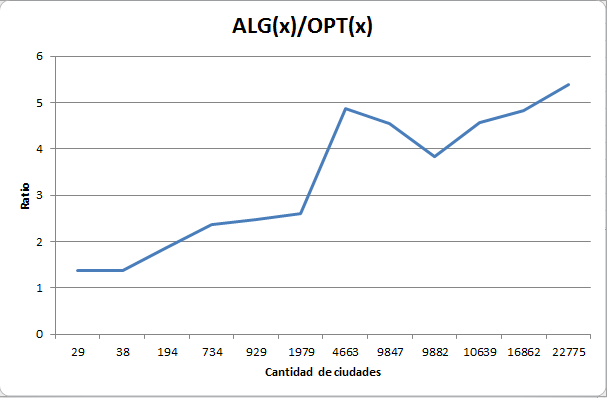
\includegraphics[scale=0.7]{img/ratioclosest.png}
 \caption{Tiempo de ejecución vs. Cantidad de ciudades}
 \end{figure}
 
  \begin{figure}[ht!]
 \centering
 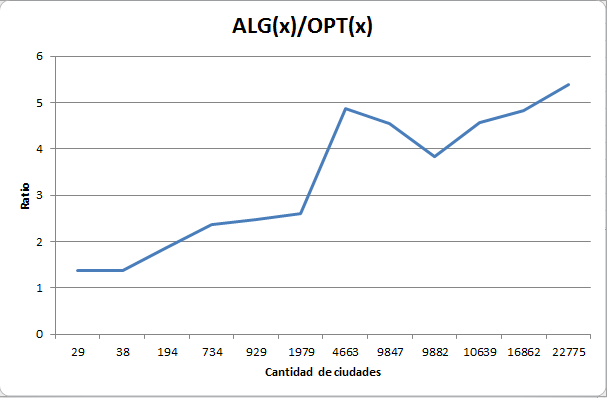
\includegraphics[scale=0.7]{img/ratioclosest.png}
 \caption{Ratio distancia algoritmo / distancia óptima}
 \end{figure}


\newpage
\section{Conclusiones}
\begin{enumerate} 
\item Efectivamente la altura de los árboles es del orden $O(\log(n))$ y además los KDTrees creados a partir de puntos de baja discrepancia poseen una menor altura, es decir la construcción es un poco más balanceada, notando que la diferencia no es completamente sustancial, pues la cantidad de nodos del árbol (espacio utilizado) es igualmente lineal.
\item La construcción de KDTrees tomó tiempo $O(n\log(n))$, tal como fue previsto. Aunque los tiempos entre los árboles con criterio $mean$ y $median$ son muy distantes, lo atribuimos al $overhead$ del cálculo de la mediana para cada conjunto de puntos, el cual es $O(n)$.
\item También se comprobó que las consultas de vecino más cercano se ejecutaron en tiempo $O(\log(n))$ para todo tipo de construcción y sin importar la distribución de puntos.
\item Se verificó que el espacio ocupado por el árbol es del orden de $O(n)$. Todos los árboles de la misma cantidad de puntos ocupan el mismo espacio, luego tienen similar o idéntica cantidad de nodos, luego la diferencia en alturas entre árboles construídos según mediana y degún media son discordantes solo por un par de ramas y no por el último nivel completo.
\item Nuestra hipótesis sobre las diferencias sobre la construcción del árbol fue errónea, dado que en la construcción del árbol el $mean$ fue mucho menor al otro, esto debido a que calcular $min$ y $max$ resultó ser más rápido que calcular la mediana..
\item Que los puntos estén distribuidos de una manera uniforme presentó leves mejoras en cuanto a los tiempos de consulta, tal como se predijo en la hipótesis, aunque esta diferencia demostró ser bastante leve.
\end{enumerate}




% ============= ANEXOS =====================
\newpage
\section{Anexos}
\subsection{Criteros de Selección de Línea de Partición}
Cadanodo, particiona el espacio según la recta que corta al eje del nivel en la mediana o en la media de la coordenada correspondiente en cada set de puntos. \\
Selección según media
\begin{lstlisting}
protected KDLine getLine(List<KDPoint> points, Axis axis) {
        return new KDLine(axis, calcMean(points,axis));  //mean between min and max of point set
    }
\end{lstlisting}
Selección según mediana
\begin{lstlisting}
protected KDLine getLine(List<KDPoint> points, Axis axis) {
        return new KDLine(axis, calcMean(points,axis));  //median calculated over groups of five
    }
\end{lstlisting}
\subsection{Vecino más cercano}
Primero se busca el nodo que marca el mismo cuadrante que el punto de consulta
\begin{lstlisting}
/*En nodos internos*/
public KDLeaf searchNeighbor(KDPoint q) {
        if(q.getCoord(line.getAxis())<= line.getPos()){
            return left.searchNeighbor(q);
        }
        else
          return right.searchNeighbor(q);
 }
 
 /* en nodos hoja*/
 public KDLeaf searchNeighbor(KDPoint q) {
        return this;  //To change body of implemented methods use File | Settings | File Templates.
}
\end{lstlisting}
Luego se busca un best fit
\begin{lstlisting}
/*En nodos internos*/
public KDLeaf anotherSearch(KDNode aChild, double currentDistance, KDPoint q) {
        KDLeaf bestLeft = new KDLeaf(new KDPoint(Double.POSITIVE_INFINITY, Double.POSITIVE_INFINITY)),
               bestRight = new KDLeaf(new KDPoint(Double.POSITIVE_INFINITY, Double.POSITIVE_INFINITY));
        if(left!=aChild && left.intersects(q,currentDistance)){
            bestLeft = left.anotherSearch(aChild, currentDistance, q);
        }
        if(right!=aChild && right.intersects(q, currentDistance)){
            bestRight = right.anotherSearch(aChild, currentDistance, q);
        }
        return (bestLeft.distance(q)>bestRight.distance(q))? bestRight:bestLeft;
}
/*En nodos hoja */
public KDLeaf anotherSearch(KDNode currentBest, double currentDistance, KDPoint q){
    if( point.distance(q)<currentDistance){
        return this;
    }
    return new KDNullNode(null);//Contiene un punto a distiancia infinita de cualquier otro
 }
\end{lstlisting}



% ============= FIN DE DOCUMENTO ==============
\end{document}

% % ················ IMAGEN ·················
% \begin{figure}[ht!]
% \centering
% \fbox{\includegraphics[scale=0.6]{img/torneo.png}}
% \caption{Torneo}\label{torneo}
% \end{figure}
% %··········································

% % ················ IMAGEN DOBLE ·················
% \begin{figure}[ht!] \centering
% \subfloat[Hola]{\includegraphics[scale=0.44]{img/holaquetal.png}}
% \subfloat[Que tal]{\includegraphics[scale=0.45]{img/holaquetal1.png}}
% \caption{Holaquetal}\label{holaquetal}
% \end{figure}
% %··········································